%% ****** Start of file apstemplate.tex ****** %
%%
%%
%%   This file is part of the APS files in the REVTeX 4 distribution.
%%   Version 4.1r of REVTeX, August 2010
%%
%%
%%   Copyright (c) 2001, 2009, 2010 The American Physical Society.
%%
%%   See the REVTeX 4 README file for restrictions and more information.
%%
%
% This is a template for producing manuscripts for use with REVTEX 4.0
% Copy this file to another name and then work on that file.
% That way, you always have this original template file to use.
%
% Group addresses by affiliation; use superscriptaddress for long
% author lists, or if there are many overlapping affiliations.
% For Phys. Rev. appearance, change preprint to twocolumn.
% Choose pra, prb, prc, prd, pre, prl, prstab, prstper, or rmp for journal
%  Add 'draft' option to mark overfull boxes with black boxes
%  Add 'showpacs' option to make PACS codes appear
%  Add 'showkeys' option to make keywords appear
%\documentclass[aps,prl,twocolumn,groupedaddress]{revtex4-1}
\documentclass[%
%reprint,
%superscriptaddress,
%groupedaddress,
%unsortedaddress,
%runinaddress,
%frontmatterverbose, 
twocolumn,
showpacs,preprintnumbers,
%nofootinbib,
%nobibnotes,
%bibnotes,
% amsmath,
 %amssymb,
 aps,
%pra,
%prb,
%rmp,
prstab,
%prstper,
%floatfix,
]{revtex4-1}
%\documentclass[aps,prl,preprint,superscriptaddress]{revtex4-1}
%\documentclass[aps,prl,reprint,groupedaddress]{revtex4-1}

% You should use BibTeX and apsrev.bst for references
% Choosing a journal automatically selects the correct APS
% BibTeX style file (bst file), so only uncomment the line
% below if necessary.
%\bibliographystyle{apsrev4-1}


\usepackage{graphics} % for pdf, bitmapped graphics files
\usepackage[pdftex]{graphicx}
\usepackage{epstopdf}
\usepackage[cmex10]{amsmath}
%\interdisplaylinepenalty=2500
\usepackage{amssymb}  % assumes amsmath package installed
%\usepackage{enumerate}
%\usepackage{setspace}
%\usepackage{verbatim}
\usepackage[colorlinks,linkcolor=blue,pdfauthor=Spencer \ Gessner,citecolor=red]{hyperref}
%\usepackage{hyperref}

\newcommand{\AFFslac}{\affiliation{SLAC National Accelerator Laboratory, Menlo Park, CA 94025, USA}}
\newcommand{\AFFucla}{\affiliation{University of California Los Angeles, Los Angeles, CA 90095, USA}}
\newcommand{\AFFoslo}{\affiliation{Department of Physics, University of Oslo, 0316 Oslo, Norway}}

\newtheorem{example}{Example}
\newtheorem{theorem}{Theorem}
\newtheorem{lemma}{Lemma}
\newtheorem{remark}{Remark}
\newtheorem{note}{Note}
\newtheorem{proof}{Proof}

\newtheorem{proposition}{Proposition}
\newtheorem{definition}{Definition}%{definition}
\newtheorem{assumption}{Assumption}
\newtheorem{corollary}{Corollary}%[section]

\begin{document}

% Use the \preprint command to place your local institutional report
% number in the upper righthand corner of the title page in preprint mode.
% Multiple \preprint commands are allowed.
% Use the 'preprintnumbers' class option to override journal defaults
% to display numbers if necessary
%\preprint{}

%Title of paper
\title{Longitudinal Phase Space Evolution and Tomographic Reconstruction at FACET}

% repeat the \author .. \affiliation  etc. as needed
% \email, \thanks, \homepage, \altaffiliation all apply to the current
% author. Explanatory text should go in the []'s, actual e-mail
% address or url should go in the {}'s for \email and \homepage.
% Please use the appropriate macro foreach each type of information

% \affiliation command applies to all authors since the last
% \affiliation command. The \affiliation command should follow the
% other information
% \affiliation can be followed by \email, \homepage, \thanks as well.
%\author{Spencer~Gessner}
\author{S.J.~Gessner}
\AFFslac

%%%%%%%%%%%%%%%%%%%%%%%%%%%%%%%%%%%%%%%
% All Other Authors (alphabetical)
\author{E.~Adli}
\AFFslac
\author{J.M.~Allen}
\AFFslac
\author{C.I.~Clarke}
\AFFslac
\author{S.~Corde}
\AFFslac
\author{F.J.~Decker}
\AFFslac
\author{A.S.~Fisher}
\AFFslac
\author{J.~Frederico}
\AFFslac
\author{M.J.~Hogan}
\AFFslac
\author{N.~Lipkowitz}
\AFFslac
\author{S.~Li}
\AFFslac
\author{M.~Litos}
\AFFslac
\author{D.~Walz}
\AFFslac
\author{G.~White}
\AFFslac
\author{V.~Yakimenko}
\AFFslac
\author{G.~Yocky}
\AFFslac

\email[]{sgess@slac.stanford.edu}
\thanks{This research was supported by DOE.}
%\affiliation{SLAC National Laboratory}

%Collaboration name if desired (requires use of superscriptaddress
%option in \documentclass). \noaffiliation is required (may also be
%used with the \author command).
%\collaboration can be followed by \email, \homepage, \thanks as well.
%\collaboration{}
%\noaffiliation

\date{\today}

\begin{abstract}
The Facility for Advanced Accelerator Experimental Tests (FACET) at SLAC provides high energy electron beams for Plasma Wakefield Acceleration (PWFA) research. PWFA experiments require high peak-current bunches in order to drive large amplitude wakes in a plasma. Creating short bunches with high charge requires a detailed understanding and control of the beam's longitudinal phase space as it evolves in the linac. In this paper, we provide an overview of the bunch compression scheme at FACET and describe a novel tomographic method that allows us to reconstruct the beam's longitudinal phase space at the end of the linac.
\end{abstract}

% insert suggested PACS numbers in braces on next line
%\pacs{41.85.Lc, 02.30.Yy, 29.20.-c, 02.60.-x}
% insert suggested keywords - APS authors don't need to do this
%\keywords{}

%\maketitle must follow title, authors, abstract, \pacs, and \keywords
\maketitle





%%%%%%%%%%%%%%%%%%%%%%%%%%%%%%%%%%%%%%%%%%%%%%%%%%%%%%%%%%%%%%%%%%%%%%%%%%%%%%%%%%%%%%%%

%%%%%%%%%%%%%%%%%%%%%%%%%%%%%%%%%%%%%%%%%%%%%%%%%%%%%%%%%%%%%%%%%%%%%%%%%%%%%%%%%%%%%%%%

\section{Introduction}
The Facility for Advanced Accelerator Experimental Tests (FACET) is designed to produce extremely high peak-current bunches for research on Plasma Wakefield Acceleration (PWFA) and other high-gradient acceleration methods~\cite{mjh_facet}. Producing a high-peak current bunch requires careful manipulation of the longitudinal phase space, so that the maximum amount of charge is packed into the shortest possible length. This process, called bunch compression, has two steps. First, an energy correlation, or chirp, is applied to the beam by an RF cavity. Second, the beam travels through a magnetic chicane where particles of different energies take different paths. A chicane is characterized by the matrix parameter $R_{56}$, which relates the change in path length of an off-energy particle relative to the on-energy trajectory. We attempt to minimize the bunch length $\sigma$ by tuning $R_{56}$ and $\delta$, the energy spread due to the chirp, such that $\sigma_f = \sigma-R_{56}\delta = 0$. Figure~\ref{bc} illustrates this balancing act.

\begin{figure}[htb]
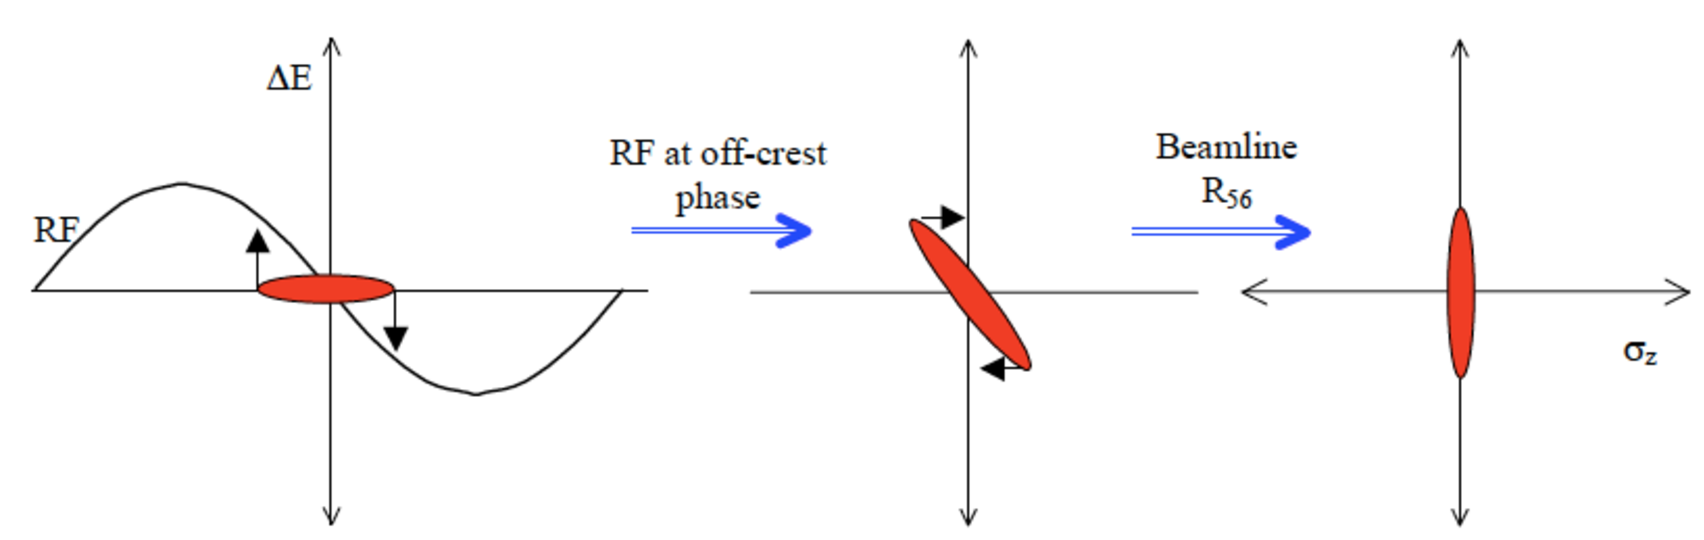
\includegraphics[width=\columnwidth]{figures/bc.pdf}
  \caption{The beam is compressed by correlating the longitudinal phase space with an RF cavity and rotating the phase space in a chicane.}
  \label{bc}
\end{figure}

In practice, we cannot reduce the bunch to zero length. The minimum bunch length is determined by the conservation of longitudinal phase space
\begin{equation}\label{cons}
 \sigma_{z_{min}} = \frac{\varepsilon_0}{\delta_f E_f}
\end{equation}
where $\varepsilon_0 = \sigma_0\delta_0 E_0$ is the initial longitudinal phase space volume. We can minimize the bunch length by maximizing the beam energy and energy spread. The beam is accelerated to a final energy of 20.35 GeV at FACET, which makes it the highest energy electron beam currently produced on Earth. The largest acceptable energy spread is about 1.7\% rms and is set by the momentum apertures of the chicanes and final focus system at FACET.

The bunch compression scheme used at FACET was first developed for the SPPS research program at the FFTB~\cite{pe_spps}. FACET uses a system of three bunch compressors to reduce the bunch length from an initial value greater than 6 mm to a final bunch length as small as 20 $\mu$m. Final compression at FACET is achieved in the W-chicane. The $R_{56}$ of the W-chicane can be tuned from 0 to 10 mm to produce different longitudinal bunch profiles. In this paper, we study the chicane in the 10 mm configuration, which is used to produce double-gaussian profiles for PWFA experiments.

The final bunch profile is sensitive to many parameters in the linac, including initial bunch length, RF chirp phase, and the $R_{56}$ of compressor chicanes. To the greatest extent possible, feedbacks are implemented to control and stabilize the beam as it evolves in the linac. Some parameters are not under feedback control, and for this reason it is critical to have real time diagnostics for the bunch length, energy spectrum, and longitudinal phase space.

FACET uses an x-band transverse deflecting cavity (TCAV) for precision bunch length measurements with temporal resolution better than 50 fs and a half-period wiggler magnet for non-destructive energy spectrum measurements. These two diagnostics measure projections of the longitudinal phase space. A third measurement was developed by creating a tunable momentum aperture, or slit, and using the TCAV and spectrometer to diagnose mono-energetic slices of the beam. By combining the bunch profiles measured for each slice, we are able to tomographically reconstruct the beam's longitudinal phase space. The tomographic phase space diagnostic is a valuable tool for optimizing double-gaussian beam structures and understanding the results of PWFA experiments.

Throughout the paper, we reference simulations of the longitudinal phase space performed with the 2D particle tracking code LiTrack~\cite{litrack}.

\begin{figure*}[htb]
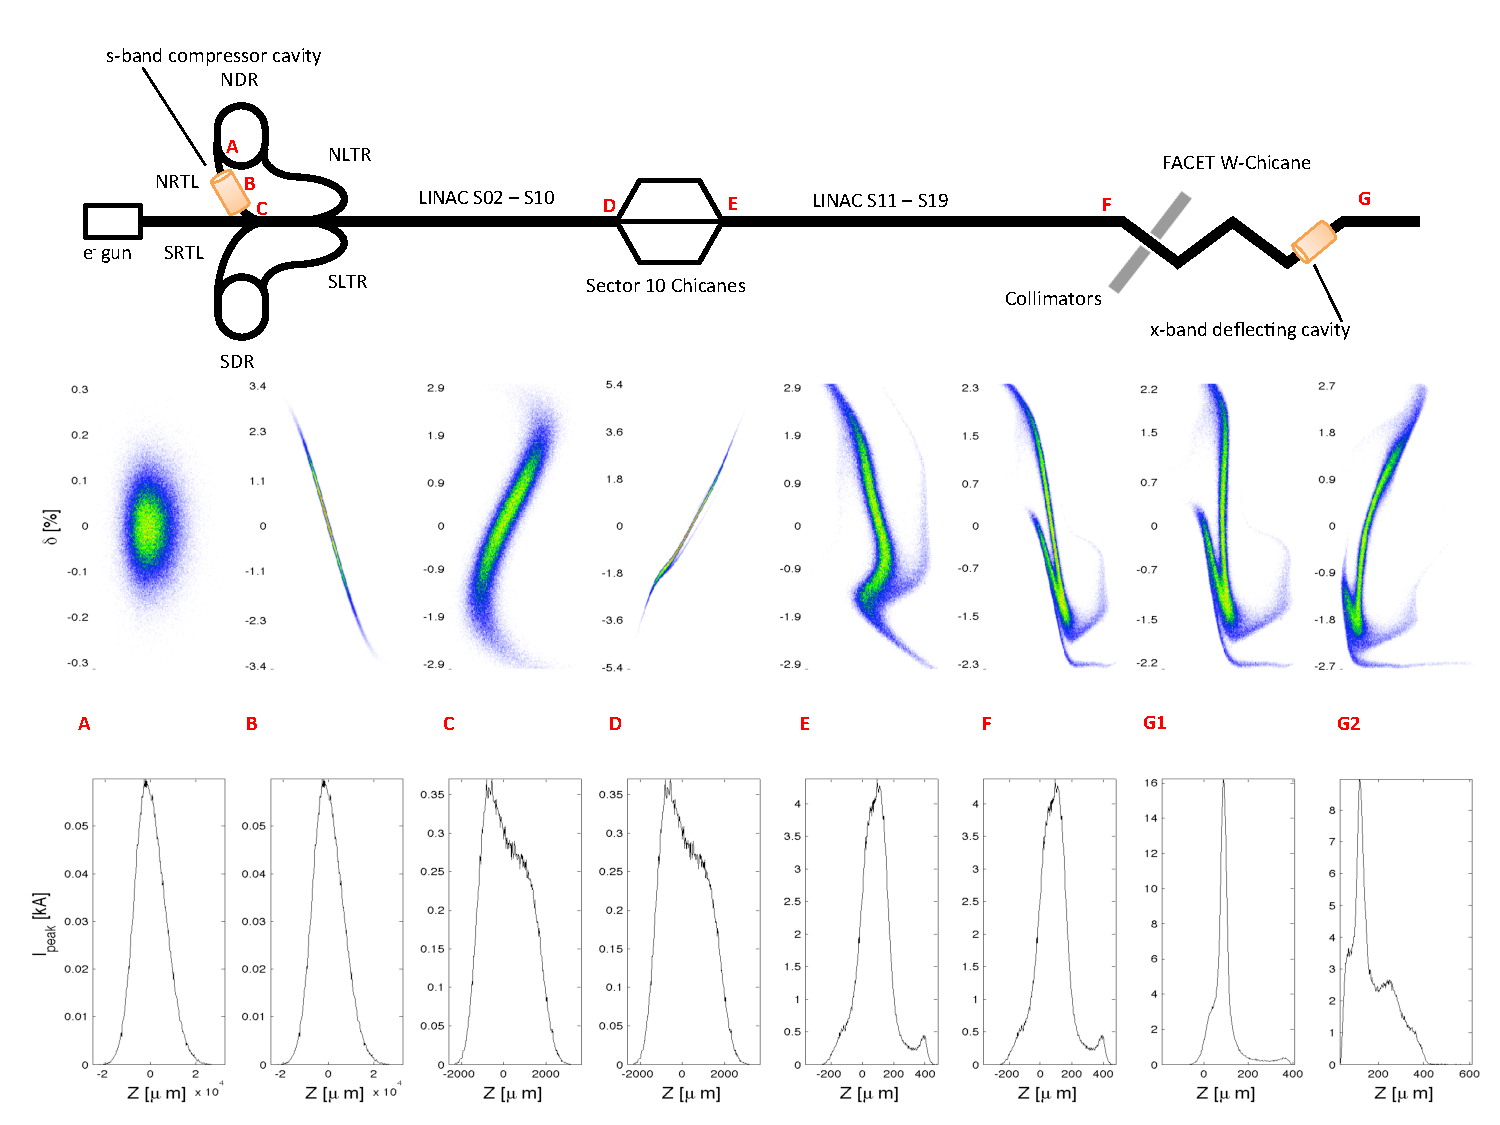
\includegraphics[width=\textwidth,height=12cm]{figures/facet_schem.pdf}
  \caption{Top: Overview of the FACET linac. Beamline elements that determine the longitudinal phase space are labeled. TCAV diagnostic and wiggler spectrometer (not shown) are located in the final leg of the W-chicane. Center: The beam phase space as simulated by LiTrack for the linac regions labeled A-G. The beam travels to the left in these plots. Bottom: The longitudinal projections (bunch profile) of the phase spaces above. G1 is the projection for the maximally compressed beam using W-chicane $R_{56} = 5$ mm. G2 shows the projection with $R_{56} = 10$ mm used for two-bunch beam profiles.}
  \label{schem}
\end{figure*}

%%%%%%%%%%%%%%%%%%%%%%%%%%%%%%%%%%%%%%%%%%%%%%%%%%%%%%%%%%%%%%%%%%%%%%%%%%%%%%%%%%%%%%%%
%The longitudinal bunch parameters prior to injection in the NDR are approximately $\sigma_z = 2.33$ mm and $\delta = 1$\% which gives a longitudinal phase space volume of $\varepsilon_{0} = \sigma_z \sigma_{\delta} = 27.73$ MeV$\cdot$mm. 
%%%%%%%%%%%%%%%%%%%%%%%%%%%%%%%%%%%%%%%%%%%%%%%%%%%%%%%%%%%%%%%%%%%%%%%%%%%%%%%%%%%%%%%%

\section{Longitudinal Phase Space Evolution in the FACET Linac}\label{sec:facet}

The FACET linac is 2 kilometers long and accelerates a 3.2 nC electron beam to a final energy of 20.35 GeV. The beam is generated from a thermionic cathode at the west end of the linac and captured by the Sector 0 RF cavities. It is accelerated to 1.19 GeV in the Sector 1 s-band cavities and is transferred to the North Damping Ring (NDR) via the North Linac to Ring chicane (NLTR). The beam is transversely and longitudinally damped in the NDR before it is extracted into the North Ring to Linac chicane (NRTL). The NRTL is the first of three bunch compressor chicanes at FACET. The beam is accelerated to 9 GeV and chirped by the RF in the first kilometer of the linac (Sectors 2-10) before being compressed again in the Sector 10 chicane. Following the Sector 10 chicane, the beam is accelerated on crest to 20.35 GeV in the second kilometer of the linac (Sectors 11-19). Beam induced wakefields provide a chirp in this portion of the beamline before the bunch undergoes final compression in the FACET W-chicane. Figure~\ref{schem} shows the beamline elements that effect the longitudinal evolution of the beam.

\subsection{North Damping Ring}\label{NDR}

The electron beam is radiatively damped to an equilibrium bunch length and an equilibrium energy spread in the NDR. The bunch is stored in the ring for 16.7 ms and the longitudinal damping time $\tau_z = 1.79$ ms. The bunch parameters out of the NDR are the initial conditions for longitudinal phase space evolution in the linac.

The radiation damping mechanism leads to a useful diagnostic for determining the initial bunch profile before the beam enters the linac. We imaged synchrotron radiation generated by the beam in one of the bends of the ring with a Hamamatsu C5680 streak camera. The camera was operated in ``synchroscan" mode, so that the bunch profile can be measured for multiple passes of the beam during the store. Figure~\ref{streak} shows the streaked beam image for the final fives turns before extraction.  The bunch is fit to an asymmetric gaussian with the form
\begin{equation}
 \lambda(z) = \frac{N_b}{\sqrt{2\pi}\sigma_z}\exp{ \left[-\frac{1}{2}\left(\frac{z}{(1\pm A)\sigma_z}\right)^2\right]}.
\end{equation}
$z = ct-s$ is the co-moving beam coordinate with the head of the beam at $z < 0$. $N_b$ is the number of beam electrons and $A$ is the asymmetry factor.  The asymmetry arrises from the distortion of the RF potential due to beam loading. The measured bunch length was $\sigma_z = 6.59$ mm, about 20\% longer than what was measured during SLC operation for similar bunch charge and RF parameters~\cite{Holtzapple}.

\begin{figure}[htb]
  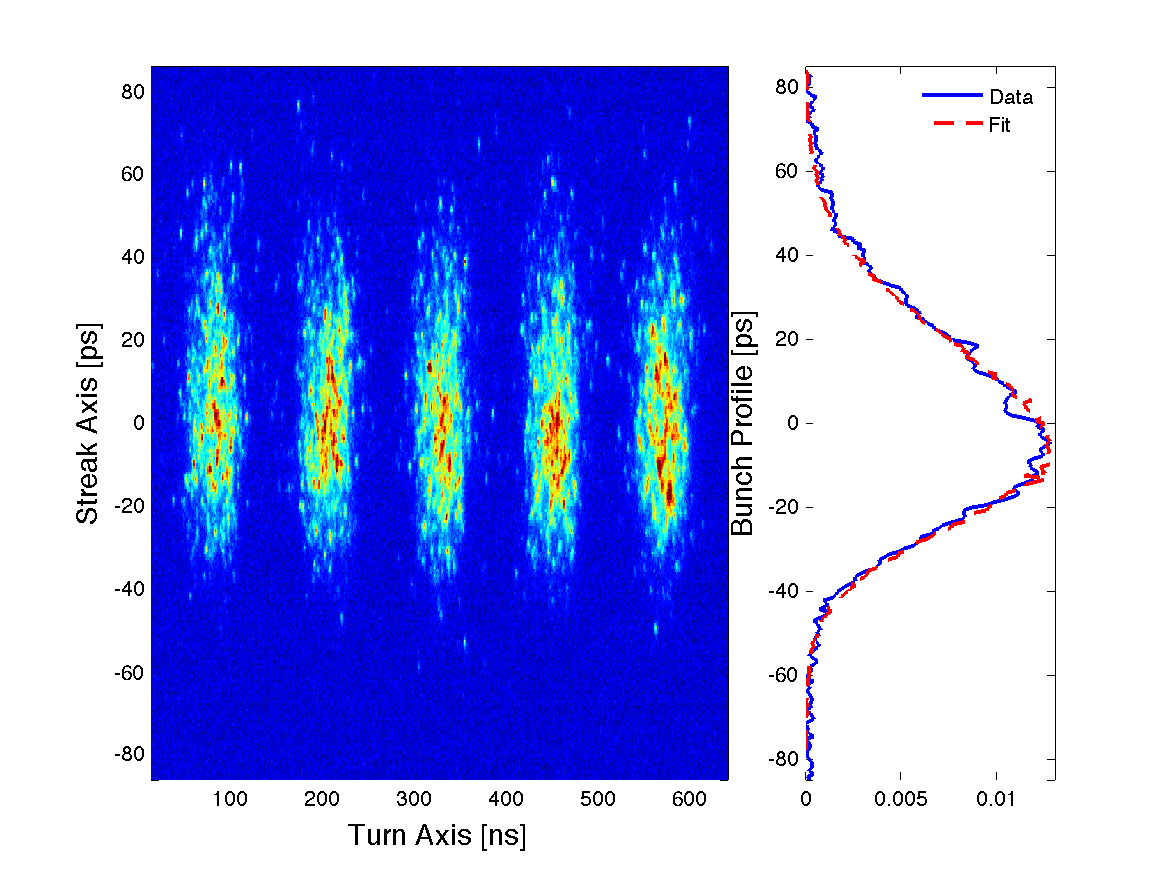
\includegraphics[width=\columnwidth]{figures/combo.pdf}
  \caption{Streak camera image of the final five turns before extraction from NDR. The bunch profile on the right is the average of the five turns shown, fit to an asymmetric gaussian with $\sigma_t = 22$ ps or $\sigma_z = 6.59$ mm, and asymmetry parameter -0.2.}
  \label{streak}
\end{figure}

The energy spread out of the damping ring has previously been measured to be $\delta = 8.3 \times 10^{-4}$~\cite{holtz_ring}. The longitudinal phase space volume out of the ring is $\varepsilon_{NDR} = 5.7$ MeV$\cdot$mm. $\varepsilon_{NDR}$ sets a lower limit on the final bunch length that can be achieved at the end of the linac.

\subsection{Chirping and Compression in the First Half of the Linac}\label{first}

The correlation in the $z-\delta$ phase space, or chirp, is defined as
\begin{equation}
C_{z\delta} = \int (z-<z>)(\delta - <\delta>)\rho(z,\delta)dzd\delta
\end{equation}
where $\rho(z,\delta)$ is the normalized longitudinal phase space density. The chirp is positive if the beam energy increases from head to tail and negative if the beam energy decreases from head to tail. 

The beam has zero chirp when it exits the NDR. Upon extraction from the ring, the beam passes through the s-band compressor cavity in the NRTL. Particles in the beam experience energy gain or loss according to
\begin{equation}
U_{RF}(z) = e E L \cos(kz + \phi)
\end{equation}
for cavity field strength $E$, cavity length $L$, RF wavenumber $k$, and cavity phase $\phi$. Cavity phase is defined such that $0^o$ is on crest and negative phases are ahead of crest, consistent with the definition of $z$ given in Section~\ref{NDR}. We can also define the chirp applied to the bunch by a beamline element as the change in energy of a particle at a position one $\sigma$ from the center of the bunch, multiplied by the distance from the center of the bunch
\begin{equation}
C_{RF} = \sigma \frac{U_{RF}(\sigma) - U_{RF}(-\sigma)}{2}.
\end{equation}
The emittance and the chirp are both measured in MeV$\cdot$mm. This definition of beamline chirp is useful because it can also be used to describe the chirp induced by wakefields in Section~\ref{wakes}.

The beam traverses the compressor cavity at the zero crossing ($\phi = 90^o$), which imposes a negative, linear chirp on the beam. The bunch is slightly over-compressed in the NRTL and exits the chicane with a residual positive chirp. Over-compression reduces beam tails, reduces the strength of wakefields, and creates a phase space with the same sign chirp as the RF chirp applied to the beam in Sectors 2-10~\cite{fj_over}. The bunch length is roughly 1.2 mm when the beam is captured in the s-band linac.
%Upon extraction from the NDR, the beam is accelerated by RF cavities in the FACET linac. The energy gain of a particle in an RF cavity is given by
%The FACET linac uses more than 500 constant gradient RF cavities to accelerate the beam to its final energy. The energy gain of a particle at position $z$ in the bunch in an RF cavity is given by
%\begin{equation}
%\Delta E_{RF}(z) = e \mathcal{E} L \cos(kz + \phi)
%\end{equation}
%for cavity field strength $\mathcal{E}$, cavity length $L$, RF wavenumber $k$, and cavity phase $\phi$. Cavity phase is defined such that $0^o$ is on crest and negative phases are ahead of crest, consistent with the definition of $z$ given in Section~\ref{NDR}. The accelerating sections can also be used to chirp the beam. We define the chirp from an accelerating section as the derivative of the energy gain evaluated at the center of the bunch, multiplied by the length of the bunch
%\begin{equation}
%C_{RF} = \sigma_z \left. \frac{d\Delta E_{RF}}{dz} \right|_{z=0} = -\sigma_z e \mathcal{E} L k \sin{\phi}.
%\end{equation}
%The chirp is positive if the energy of the beam particles increases with $z$. This is a useful definition of chirp because it can be applied to both RF phase chirping and the longitudinal wakefield chirping described in Section~\ref{wakes}.

%Immediately after extraction from the NDR, the electron beam passes through the s-band compressor cavity in the North Ring to Linac (NRTL) chicane. The compressor cavity applies a negative, linear chirp to the beam. The bunch is slightly over-compressed in the NRTL and exits the chicane with a residual positive chirp. Over-compression reduces beam tails, reduces the strength of wakefields, and creates a phase space with the same sign chirp as the RF chirp applied to the beam in Sectors 2-10. The bunch length is roughly 1.2 mm when the beam is captured in the s-band linac.

%The beam is compressed by a factor of 10 in the North Ring to Linac (NRTL) chicane and enters the Linac with a 600 $\mu$m RMS bunch length. The bunch is slightly over-compressed, with a residual low-to-high chirp, so as to minimize the impact of wakefields in the linac. 

\begin{figure}[hb]
  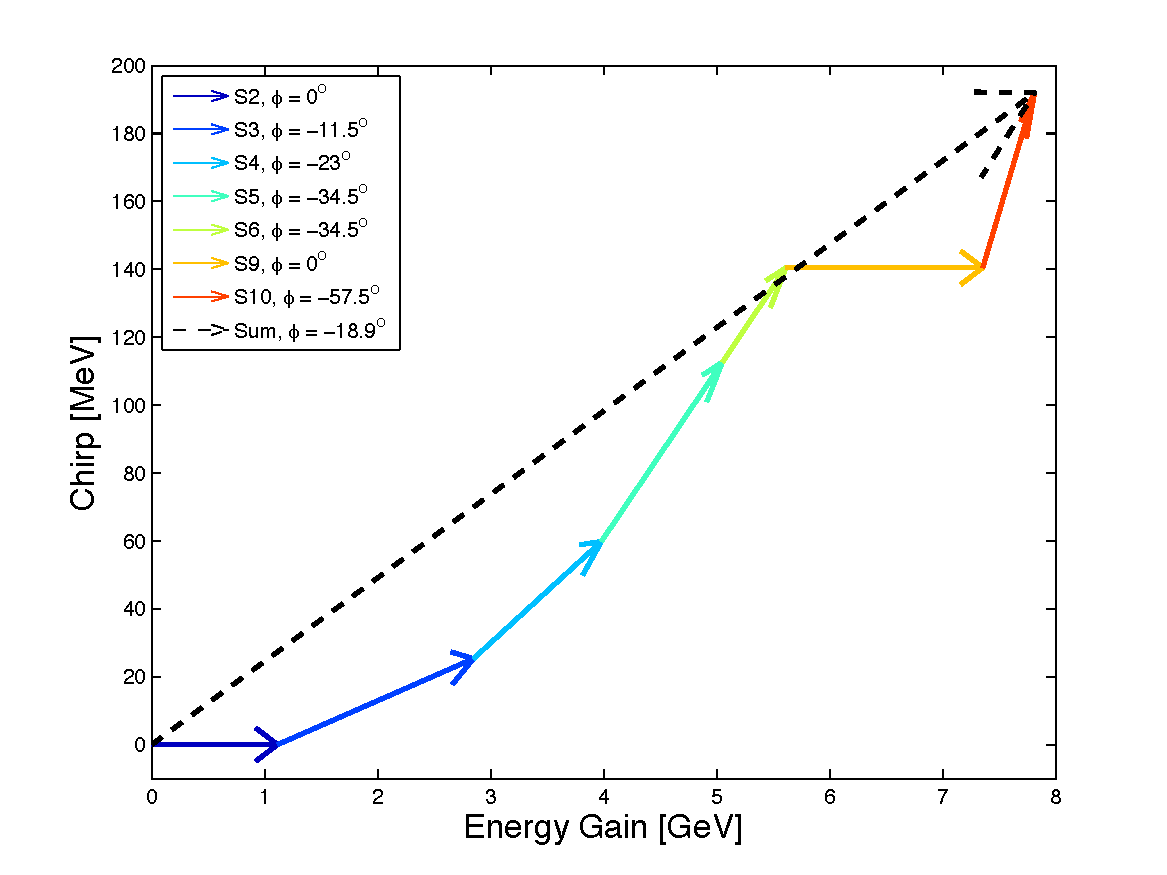
\includegraphics[width=\columnwidth]{figures/chirp_plot.pdf}
  \caption{Diagram showing the phasing in sectors 2-10 at FACET. Each arrow represents the phase and amplitude of the accelerating sector. Sectors 7 and 8 are not operational.}
  \label{stag}
\end{figure}

The bunch is accelerated in the first kilometer of the linac with a net phase of about -20 degrees. FACET uses a unique chirping scheme in the front end of the linac that staggers the RF chirp phase over five linac sectors. The staggered chirp process is depicted in Figure~\ref{stag}. By accelerating on crest or nearly on crest in the first few sectors, the beam becomes stiff and is resistant to emittance dilution from transverse wakefields. The later sectors have stronger phasing, up to -55 degrees off crest, in order to achieve an average of -20 degrees chirp prior to the Sector 10 Chicane. While this scheme has the advantage of reducing emittance growth, it makes the beam more sensitive to phase errors in the highly chirped sectors.

The bunch length is compressed from 1.2 mm to less than 100 $\mu$m in the Sector 10 chicane. The bunch is slightly over-compressed, with residual negative chirp.

\subsection{Wakefield Chirping and Compression in the W-Chicane}\label{wakes}

The high-charge electron bunch is extremely short compared to the RF wavelength after compression in the Sector 10 chicane. The bunch length is less than 0.5 s-band degrees, making it impractical to use the RF to simultaneously accelerate and chirp the beam. On the other hand, the peak current for the electron bunch is over 4 kA and drives a large amplitude, longitudinal wakefield in the RF cavities, which can be used to chirp the beam. The energy change of a particle at position $z$ in the bunch is given by
\begin{equation}
U_W = L \int_0^\infty \lambda(z-z')W(z')dz'
\end{equation}
where $L$ is the total length of RF cavities traversed by the beam, $\lambda(z)$ is the longitudinal charge distribution, and $W(z)$ is the single particle Green's function for the SLAC s-band cavity. The wake function comes from a numerical time domain simulation of the SLAC s-band cavity. In addition, analytical formulae were developed to estimate the average energy loss (wake loss) of the bunch as a function of bunch length. Both the numerical and analytical results have been benchmarked with experimental data~\cite{sup_short}\cite{novo}.

\begin{figure}[hb]
  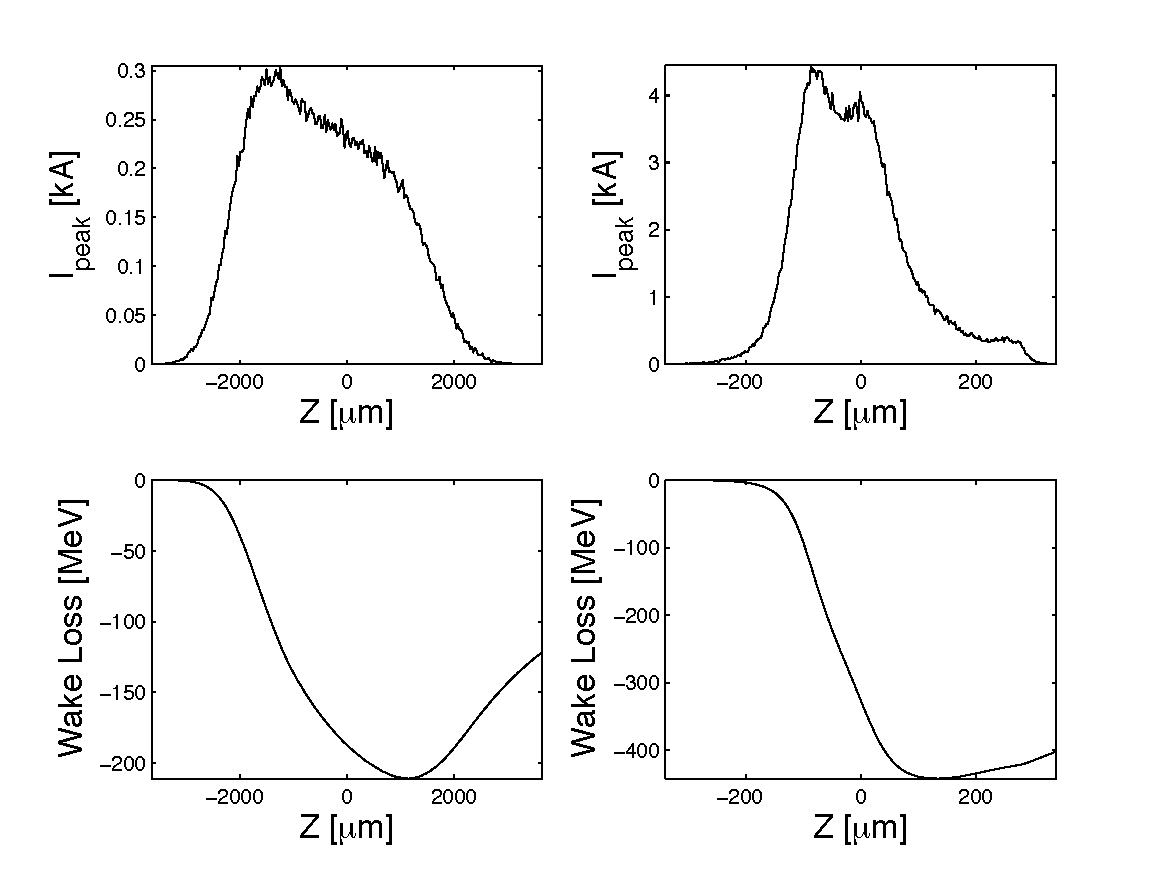
\includegraphics[width=\columnwidth]{figures/wakeloss.pdf}
  \caption{The bunch profile and wake loss for the first and second kilometers of the FACET linac.}
  \label{wake}
\end{figure}

The chirp applied to the bunch by a longitudinal wake is given by 
%\begin{equation}
%C_{W} = \sigma_z \left. \frac{d\Delta E_{W}}{dz} \right|_{z=0}
%\end{equation}
\begin{equation}
C_{W} = \sigma \frac{U_{W}(\sigma) - U_{W}(-\sigma)}{2}.
\end{equation}
analogous to the RF phase chirp defined in Section~\ref{first}. Figure~\ref{wake} shows the energy loss due to beam induced wakefields, or wake loss, in the first and second kilometer of the FACET linac. For very short bunches, the wakefield is approximately linear across the core of the bunch, and is therefor an effective method for chirping the beam prior to final compression in the FACET W-Chicane.

%Again, the bunch is over-compressed, this time with a residual high-to-low chirp. The very short (50 $\mu$m), very high charge (3.2 nC) bunch drives a high-amplitude longitudinal wakefield in the SLAC s-band cavities. The wakeloss function $W(z)$ is a convolution of the cavity wake structure and the bunch profile, but for very short bunches it is roughly linear over the core of the bunch. The net effect of the wakefields in the second kilometer of the linac is to provide a mostly linear high-to-low chirp that will be leveraged for bunch compression in the FACET W-Chicane.

The FACET W-Chicane is a unique lattice that features adjustable $R_{56}$.  When extremely short bunches are needed, the chicane is tuned to $R_{56} = 5$ mm and yields a gaussian bunch with $\sigma_z = 20~\mu$m. For the two-bunch setup, the $R_{56} = 10$ mm, which over-compresses the bunch with a residual low-to-high chirp. 

Table~\ref{dat_table} lists beamline parameters and chirp at different points in the linac.

\begin{table}
  \begin{tabular}{ l c c c c c c}
    \hline
    Element & $R_{56} $[mm] & $\phi_{rf}$ & $\sigma_z$[$\mu$m] & $C_{z\delta}$ & $C_{RF}$ & $C_{W}$ \\ \hline
    NDR &  & & 6600 & 0 & & \\
    NRTL Cavity &  & $ 90^o$ & 6600 & -80 & -86.8 & -0.33 \\
    NRTL Chicane & 602.6 & & 1200 & 14.05 &  & \\
    S02-10 &  & $-20^o$ & 1200 & 172.63 & 228.6 & -77.95 \\
    S10 Chicane & -75.8 & & 50 & -7.46 & & \\
    S11-19 & & $0^o$ & 50 & -17.69 & -0.04 & -15.63 \\
    W-Chicane & 5 & & 20 & 0.022 & & \\
    \hline
  \end{tabular}
   \caption{Table of linac parameters and bunch lengths for each linac element. $C_{z\delta}$, $C_{RF}$, and$C_{W}$ are all measured in MeV$\cdot$mm.}
   \label{dat_table}
\end{table}

%In this case, the uncollimated bunch is non-gaussian with an RMS of 100-200 $\mu$m. A thin tantalum blade, referred to as the notch collimator, is inserted into the beam at a point where the ratio $\eta \delta / \sqrt{ \beta \varepsilon}$ is maximized early in the chicane. The notch collimator removes charge from the core of the energy spectrum, which corresponds to center of the bunch profile as a result of the $z-\delta$ correlation. Jaw collimators are used to remove high and low energy tails that lack $z-\delta$ correlation. This improves the final contrast of the two-bunch longitudinal profile.



%\begin{figure}[hbt]
%  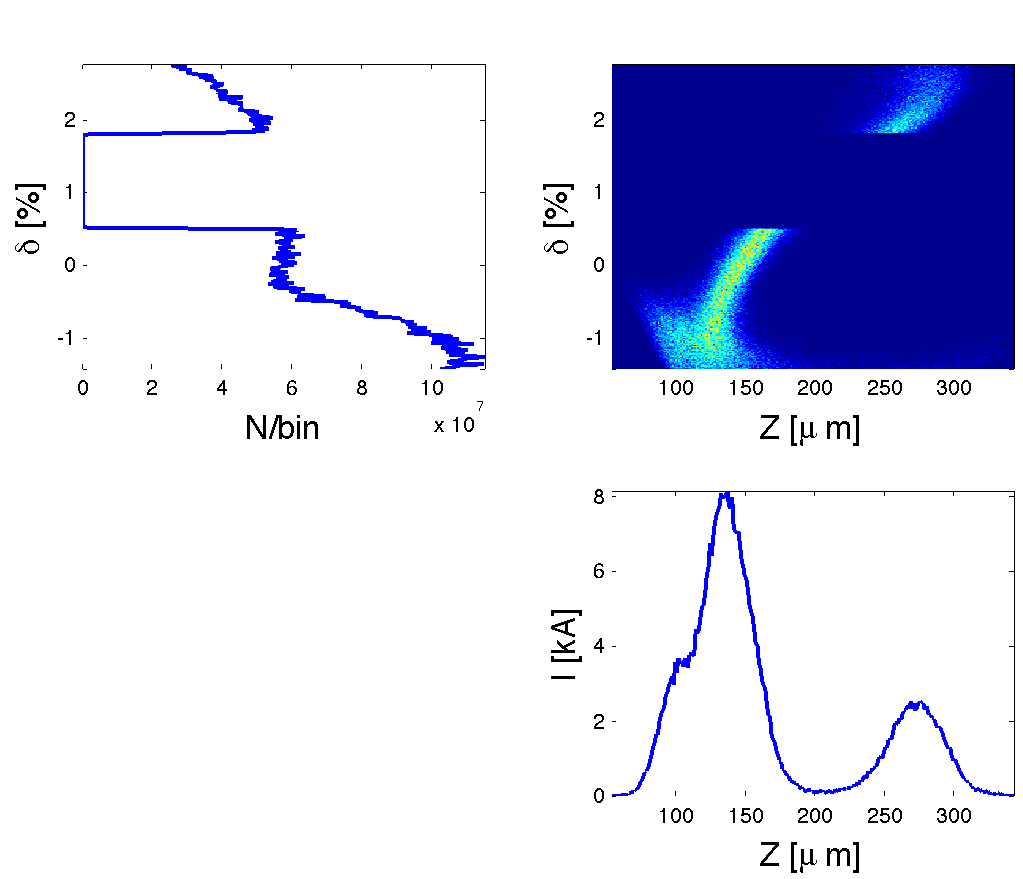
\includegraphics[width=\columnwidth]{figures/sect20.pdf}
%  \caption{LiTrack simulation of the longitudinal phase space after collimation and compression in the W-Chicane.}
%  \label{sect20}
%\end{figure}

%%%%%%%%%%%%%%%%%%%%%%%%%%%%%%%%%%%%%%%%%%%%%%%%%%%%%%%%%%%%%%%%%%%%%%%%%%%%%%%%%%%%%%%%

%%%%%%%%%%%%%%%%%%%%%%%%%%%%%%%%%%%%%%%%%%%%%%%%%%%%%%%%%%%%%%%%%%%%%%%%%%%%%%%%%%%%%%%%

\section{Diagnostics}\label{sec:diag}
A transverse deflecting x-band cavity (TCAV) is located near the end of the W-Chicane, close to maxima in $\beta_y$. The TCAV is used as a vertical streaking device; electrons with different longitudinal positions $z$ in a bunch experience different transverse deflecting fields. The particles are displaced vertically according to
\begin{equation}
\Delta Y = R_{34}\frac{e V_{rf}}{E_0}\sin{kz}
\end{equation}
and $R_{34}$ is the matrix element between the TCAV and the location where the streaked beam is imaged on a screen. The TCAV phase is calibrated such that the position $z=0$ in the beam corresponds to the zero crossing of the deflecting wave. The TCAV is the only diagnostic that has been used experimentally to resolve femtosecond beam structures. However, the TCAV is a destructive diagnostic, so it is not used while taking experimental data with plasma.

A half-period wiggler magnet is located just downstream of the TCAV at a dispersive point with the same $\eta$ and $\beta$ as the notch collimator. The wiggler deflects the horizontally-dispersed beam vertically. This generates a streak of synchrotron x-rays which are intercepted by a scintillating YAG:Ce crystal millimeters above the beam path. The x-ray streak encodes the energy spectrum of the beam onto the crystal, which is imaged by a CCD camera. On average, each 20.35 GeV electron radiates away 67 KeV of x-rays Emittance dilution due to ISR and CSR is negligible, so we the wiggler/YAG energy spectrometer is non-destructive. This is a particularly useful diagnostic, because it provides information about the longitudinal phase space on every shot.

\section{Tomographic Phase Space Reconstruction}\label{sec:tomo}
An ideal phase space measurement allows for the entire beam phase space to be imaged in a single shot. For instance, the LCLS TCAV streaks the beam horizontally before the beam passes through a vertical dipole, so that $Z\rightarrow X$ and $\delta \rightarrow Y$. The beam is imaged on a screen at a point of large $R_{15}$ and large $R_{36}$. Using this method, the longitudinal phase space is determined for every shot. 

%projects the beam's longitudinal profile and energy spectrum into the $XY$ plane so that the phase space can be imaged optically. 

At FACET, it is not possible to streak and disperse the beam in orthogonal planes without significant changes to the chicane and final focus optics. Instead, we have developed a technique that allows us to tomographically reconstruct the beam's longitudinal phase space.  We use the jaw collimators at the beginning of the FACET chicane to create a narrow slit and use the TCAV to streak the portion of the beam that passes through the slit. The collimators are located in a region with good dispersive contrast, where the ratio $\eta \delta / \sqrt{\beta \varepsilon}$ is at a maximum, so the slit acts as a momentum aperture. The collimators are scanned across the path of the dispersed beam while maintaining a constant slit width of roughly 180 $\mu$m or $\Delta E/E = 0.25\%$. The longitudinal bunch profile is recorded for each position of the slit and each profile represents the $z$-distribution of the bunch at a given $\delta$. Figure~\ref{slit} shows the measured energy spectrum of the beam with the collimators open and with the slit in place and Figure~\ref{tcav_slit} shows the same shots measured by the TCAV.

\begin{figure}[hbt]
  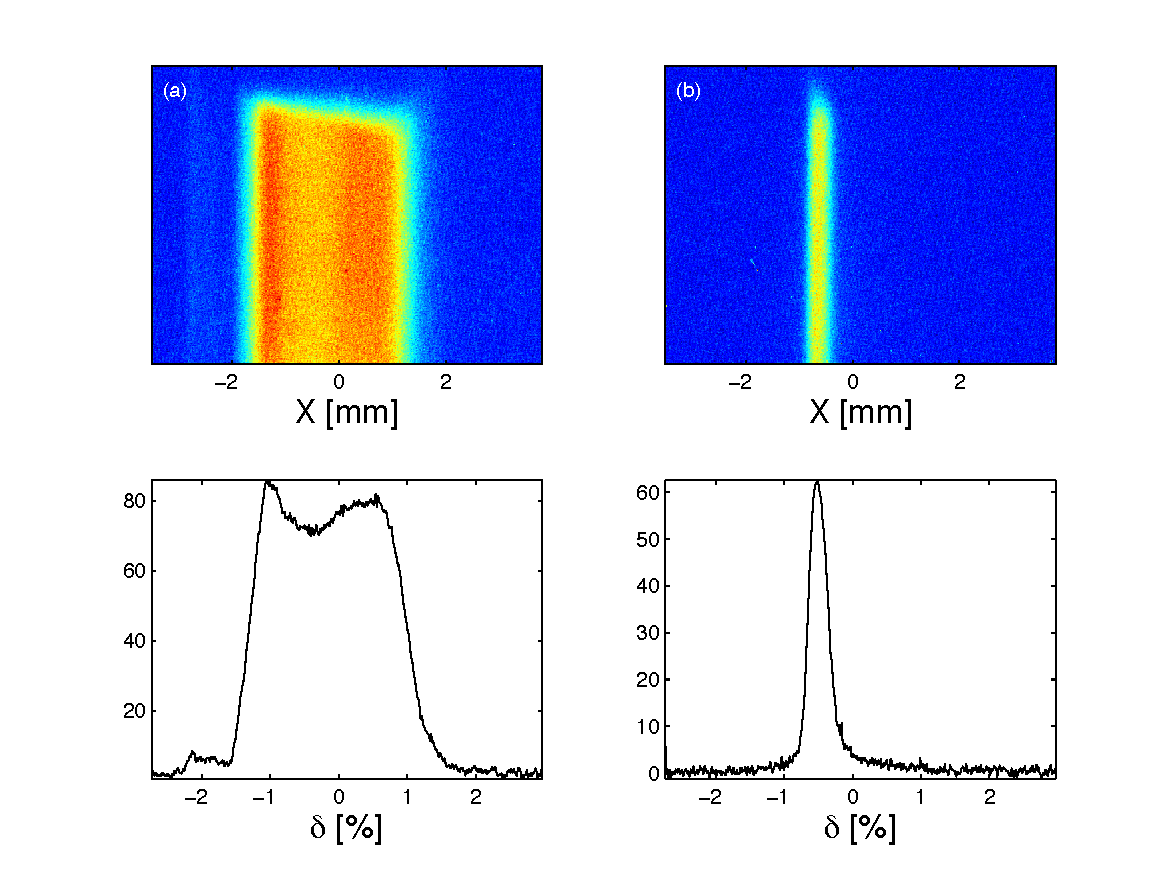
\includegraphics[width=\columnwidth]{figures/slit_wlabel.pdf}
  \caption{(a) The full beam energy spectrum imaged at the wiggler spectrometer. (b) The partial energy spectrum with the slit acting as a momentum aperture. The dispersion was measured to be 128 mm at this location.}
  \label{slit}
\end{figure}

\begin{figure}[hbt]
  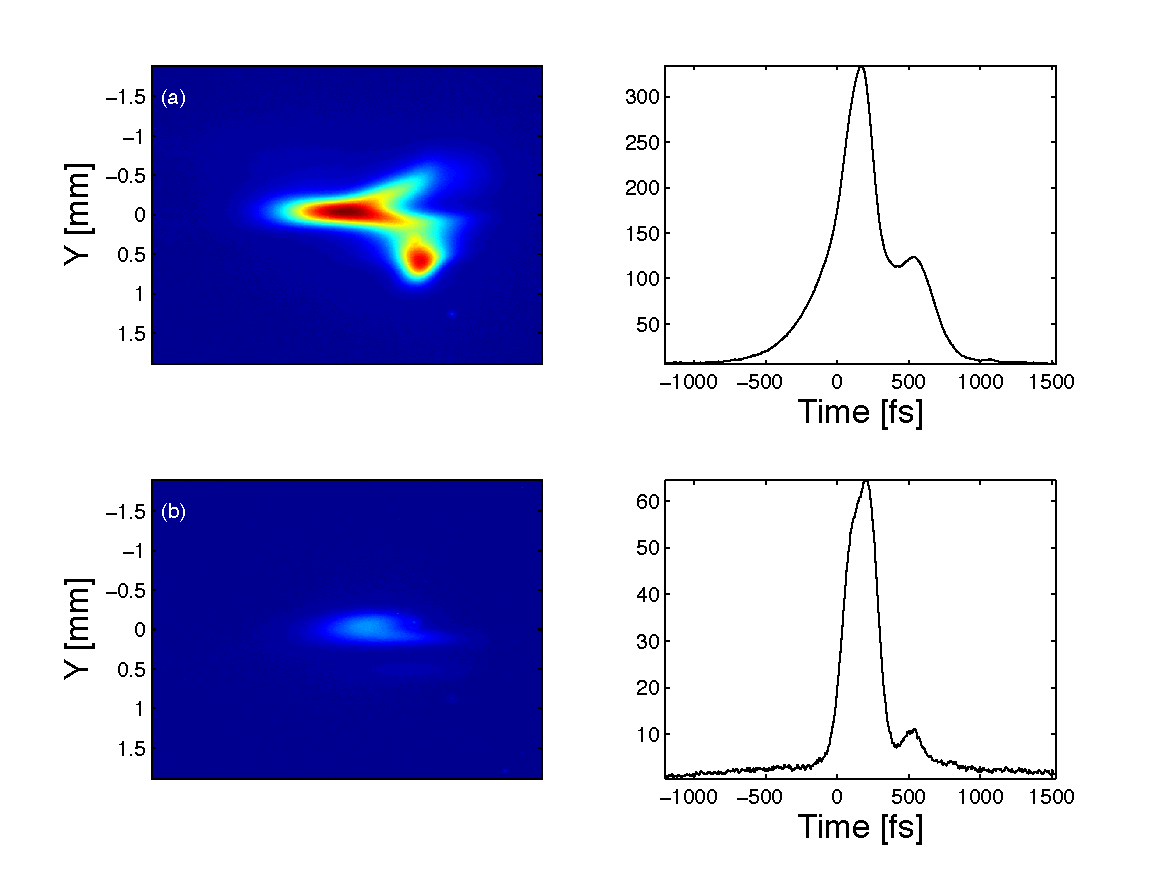
\includegraphics[width=\columnwidth]{figures/tcav_slit2.pdf}
  \caption{(a) The full bunch profile as measured with the TCAV. (b) The bunch profile measured for a monoenergetic beam slice.}
  \label{tcav_slit}
\end{figure}

There is an arrival time jitter of the beam relative to the RF phase of the TCAV. The shots in this dataset have an RMS jitter of 124 fs. By taking multiple shots per slit position, we can find an average temporal position of the profiles. Each set of 20 shots is aligned to the average position. The profiles for each slit position are stacked together to reconstruct the longitudinal phase space. Figure~\ref{raw_data} shows the raw data from a measurement taken for 10 slit positions with 20 shots each

\begin{figure}[hbt]
  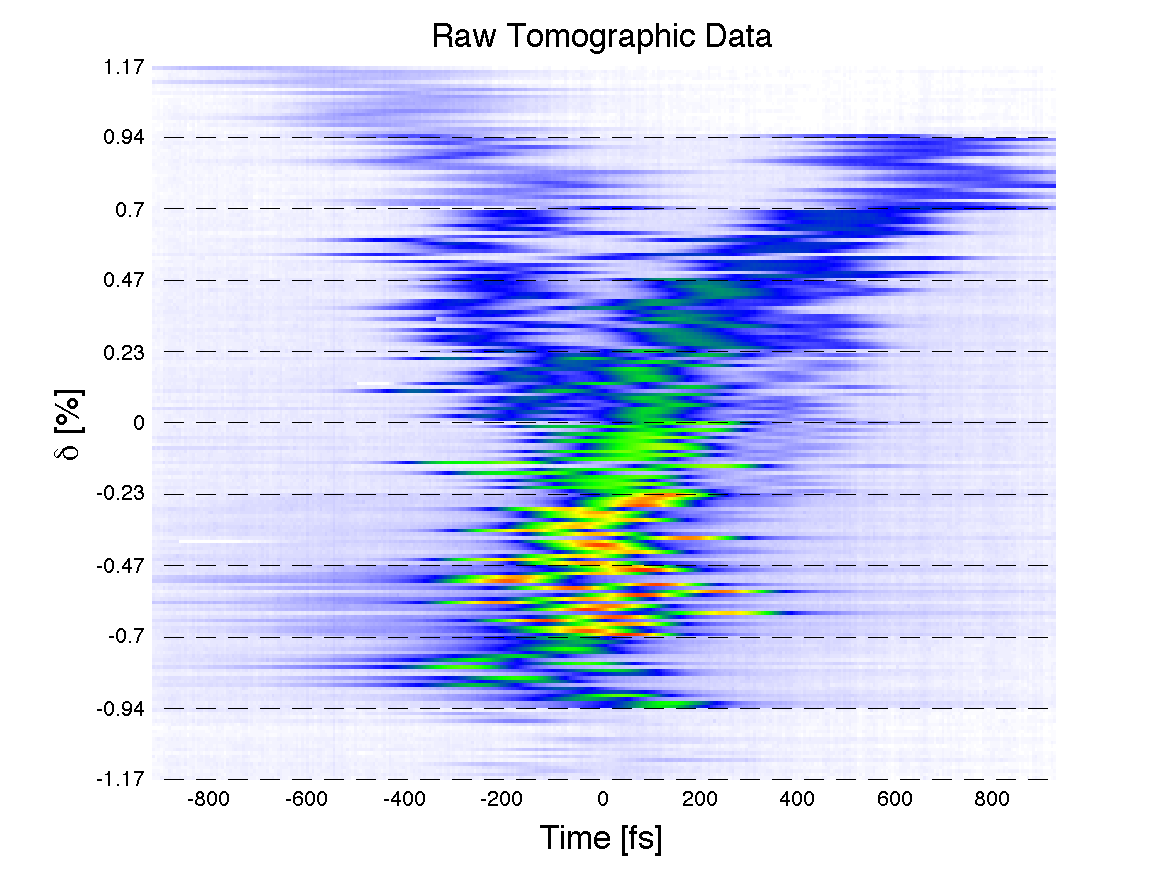
\includegraphics[width=\columnwidth]{figures/raw.pdf}
  \caption{Raw data from the tomographic slit scan measurement. Note that the $\delta$ axis is not continuous. The dashed black lines denote consecutive shots for each slit position.}
  \label{raw_data}
\end{figure}

\begin{figure}[hbt]
  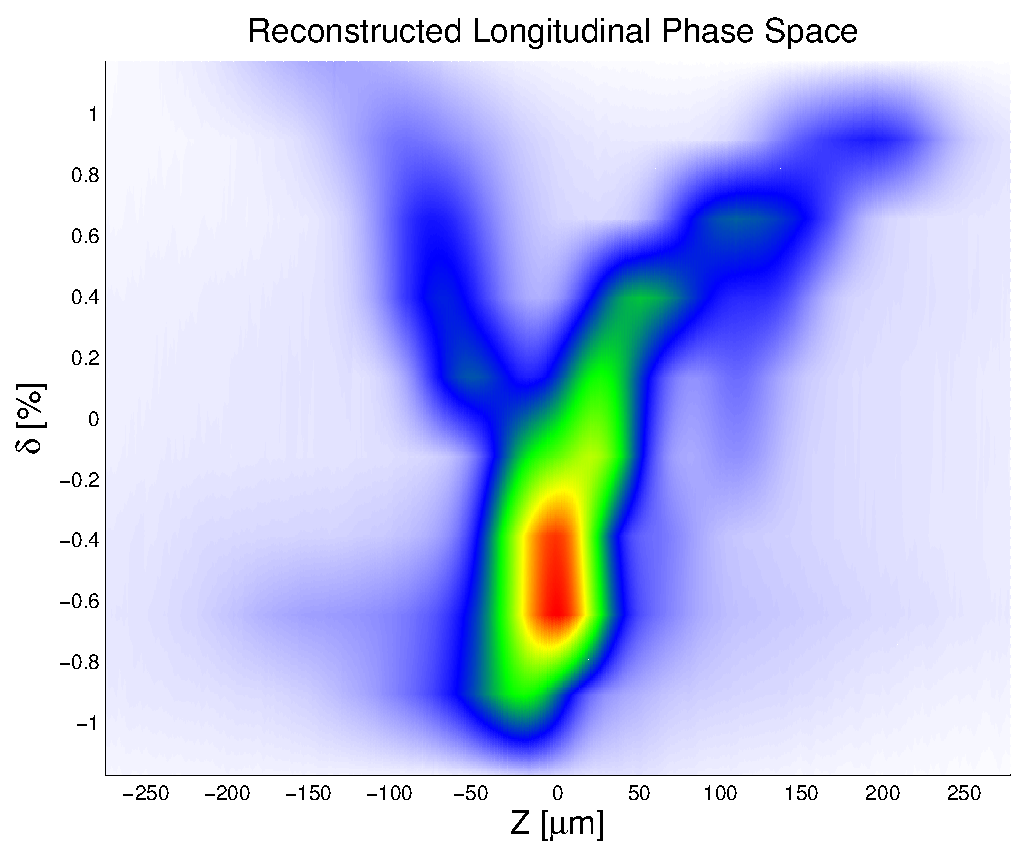
\includegraphics[width=\columnwidth]{figures/test.pdf}
  \caption{Raw data from the tomographic slit scan measurement.}
  \label{ps}
\end{figure}

\section{Comparison with Simulation}
The reconstructed phase space was compared to LiTrack simulations to determine the machine parameters that produced the bunch. We find that the bunch length in the NDR, the NRTL compressor cavity voltage, and the phase in Sectors 2-10 all had to be adjusted away from their readback values in order to make a meaningful comparison.


\section{Conclusions and Future Work} \label{sec:con}
Longitudinal phase space reconstruction is a critical tool for beam tuning and understanding the results of ongoing experiments at FACET

%%%%%%%%%%%%%%%%%%%%%%%%%%%%%%%%%%%%%%%%%%%%%%%%%%%%%%%%%%%%%%%%%%%%%%%%%%%%%%%%%%%%%%%%

%%%%%%%%%%%%%%%%%%%%%%%%%%%%%%%%%%%%%%%%%%%%%%%%%%%%%%%%%%%%%%%%%%%%%%%%%%%%%%%%%%%%%%%%



\begin{thebibliography}{99}

\bibitem{mjh_facet} M. J. Hogan et al., New J. Phys. 12, 055030 (2010).

\bibitem{pe_spps} M. Cornacchia et al., SLAC-PUB-8950.

\bibitem{litrack} P. Emma and K. Bane, SLAC-PUB-11035.

\bibitem{Holtzapple} R. Holtzapple, Ph.D. Thesis, Stanford University (1996).

\bibitem{holtz_ring} R. Holtzapple et al., SLAC-PUB-6834.

\bibitem{fj_over} F.J. Decker et al., SLAC-PUB-6604.

\bibitem{sup_short} K. Bane et al., SLAC-PUB-9905.

\bibitem{novo} A. Novokhatski, NIM A (2012).

\end{thebibliography}


\end{document}


